
\subsection{Experimental data sets}\label{sec:data}

This measurement uses data sets of \epem collisions produced by the SuperKEKB accelerator and collected by the Belle II detector in 2019-2021.
There are two data-collection modes in Belle II:
\begin{itemize}
    \item \textit{on-resonance data}: data sets collected at the collision energy $\sqrt{s}\approx10.58~\gev$, corresponding to the mass of \FourS meson;
    \item \textit{off-resonance data}: data sets collected 60~\mev below the on-resonance threshold. 
    Such data, by definition, does not contain $\BB$ events and is an excellent testing and validation sample to understand continuum processes.
\end{itemize}
The integrated luminosity, henceforth denoted as $\int~\hspace{-7pt}~\mathcal{L}$, corresponding to the on(off)-resonance sample is 189(18)~\invfb.
The on-resonance data set contains approximately $198$ million \BB pairs.

\subsection{Simulated data sets}\label{sec:MC}

In order to prepare the analysis procedure, calculate the signal-selection efficiencies and perform a validation adhering to the principles of a blinded-analysis, 
large simulated samples are utilised.
These samples are significantly larger than the data sets that were anticipated to be analysed by this analysis to ensure that uncertainties due to limited simulation samples are minimal.
The overview of the samples is discussed in this subsection, but a quick overview is provided in \Cref{tab:simulated_samples}

\begin{table}[htbp!]
    \centering
\caption{\label{tab:simulated_samples}The overview of simulated samples used in the measurement described by this thesis.
More in-depth discussion for each sample is present in the text.}
\resizebox{0.7\textwidth}{!}{
\begin{tabular}{lcc}

Simulated sample & Size  & Generators used \\ 
\hline
Generic-\Bz & \multirow{6}{*}{1+0.6~\invab}& \multirow{2}{*}{\texttt{EvtGen} \cite{Ryd:2005zz} }\\
Generic-\Bp &                          &\\
\cline{3-3}
continuum \uubar &                     & \multirow{4}{*}{\texttt{KKMC} \cite{Ward:2002qq} interfaced to Pythia 8 \cite{Sjostrand:2007gs}}\\
continuum \ddbar &                     &\\
continuum \ccbar &                     &\\
continuum \ssbar &                     &\\
\cline{2-3}
\BptoXsgamma      & \multirow{2}{*}{100 million}  & \multirow{2}{*}{\texttt{EvtGen}, \texttt{BTOXSGAMMA} model \cite{Ryd:2005zz}}\\
\BztoXsgamma      & & \\
\cline{2-3}
\Bp\to\Kstarp(782)\g    & \multirow{2}{*}{10 million} & \multirow{2}{*}{\texttt{EvtGen}, \texttt{SVP\_HELAMP} model \cite{Ryd:2005zz}}\\
\Bz\to\Kstarz(782)\g    &  & \\
\end{tabular}
}
\end{table}

All the simulated samples correspond to the 14th official Belle II simulation production campaign, and are based on Monte-Carlo methods.
Therefore, I will henceforth refer to the simulated samples as \MC.
For the analysis I use:
\begin{itemize}
    \item four \epem\ra\qqbar ($\q\in\{\u,\d,\s,\c\}$) simulated sample categories, referred to as continuum \MC,
    \item two \FourS\ra\BB categories for charged and neutral \B modes, referred to as generic-$B$ \MC.
\end{itemize}
Altogether, the above to categories are referred to as \textit{generic} \MC.
Normally, \epem\ra\tautau events are also considered as background, however when using hadronic tagging this type of background is observed to be supressed to negligible levels.

The analysis will be performed on 1.6~\invab of simulation, which is more than 6 times larger than the on-resonance data set for this analysis.
For the background subtraction step described in \Cref{sec:background_subtraction}, which has the strongest dependance on limited-\MC sample size, a significantly larger dataset is crucial.

The generic-\B \MC includes \BtoXsgamma decays, however the number of such events is expected to be small, further diminished by the efficiency of the hadronic-tagged analysis procedure, as discussed in \Cref{sec:had_tagged_overview}.
For this reason we utilise additional samples:
\begin{itemize}
    \item 100 million \BpBm sample, where at least one $B$ is guaranteed to decay as \BptoXsgamma based on the Kagan-Neubert model \cite{Kagan:1998ym} (see \Cref{sec:btosgamma_spectrum_theory});
    \item 100 million \BzBzb sample, where at least one $B$ is guaranteed to decay as \BztoXsgamma based on the Kagan-Neubert model \cite{Kagan:1998ym} (see \Cref{sec:btosgamma_spectrum_theory});
    \item 10 million \BpBm sample, where at least one $B$ is guaranteed to decay as \Bpm\ra\Kstarpm\gamma~based on the \texttt{EvtGen SVP\_HELAMP} model \cite{Ryd:2005zz};
    \item 10 million \BzBzb sample, where at least one $B$ is guaranteed to decay as \Bz\ra\Kstarz\gamma~based on the \texttt{EvtGen HELAMP} model \cite{Ryd:2005zz}.
\end{itemize}
The first two are used for general analysis setup in 
\Cref{sec:event_reconstruction,sec:photon_selection,sec:continuum_suppression,sec:final_optimisation,sec:tag_selection} and similar studies.
The $B\to\Kstar\gamma$ samples will be combined in with \BtoXsgamma in a hybrid-model approach \cite{Ramirez:1989yk} discussed in \Cref{sec:signal_model}.

In all cases, the detector response and readout is simulated using Geant 4 \cite{GEANT4:2002zbu}.

\subsection{Signal model}\label{sec:signal_model}

As it was introduced in \Cref{sec:btosgamma_spectrum_theory}, inclusive decay models, by design, assume quark-hadron duality and therefore do not describe specific resonances, but a smooth spectrum.
For \BtoXsgamma, given the experimental resolution, as well as the fact that many different decay resonances combine and interefere this is an excellent approximation.

A model based on all measured resonances (\Cref{tab:btosgamma_bfs}), that is included in the Belle II official \MC for generic-$B$ is shown in \Cref{fig:generic_Xs_model}.
The generic-$B$ model includes exclusive resonances based on their branching-fractions given in \Cref{tab:btosgamma_bfs} and scales down the Kagan-Neubert model globally to account for the inclusion of these.
There are several resonances included (those that have been observed) in the generic-$B$ model, but it can be seen their individual sharp structure is largely smoothed-out, even without experimental smearing.
On the other hand, the $B\rightarrow\Kstar(892)\gamma$ is isolated and sharply peaking.
Although this model proves a slightly better explanation of the high-\EB region, it fails at the tail region: there the inclusive model gets scaled down much lower than predicted by the inclusive model.
This is due to the fact that a global scaling is applied to \BtoXsgamma, whereas most of the added resonances lie in the high-\EB region (resonances at lower-\EB have not yet been observed).
Furthermore, the generic-$B$ model uses older \BtoXsgamma photo-energy spectrum parameters $m_b$ and $\lambda_1$ (see \Cref{sec:btosgamma_spectrum_theory}), which makes the spectrum description suboptimal.

\begin{figure}[htbp!]
    \subcaptionbox{\label{fig:generic_Xsp_model}}{
    \clipbox*{{0.0\width} {0\height} {0.5\width} {1\height}}{%
    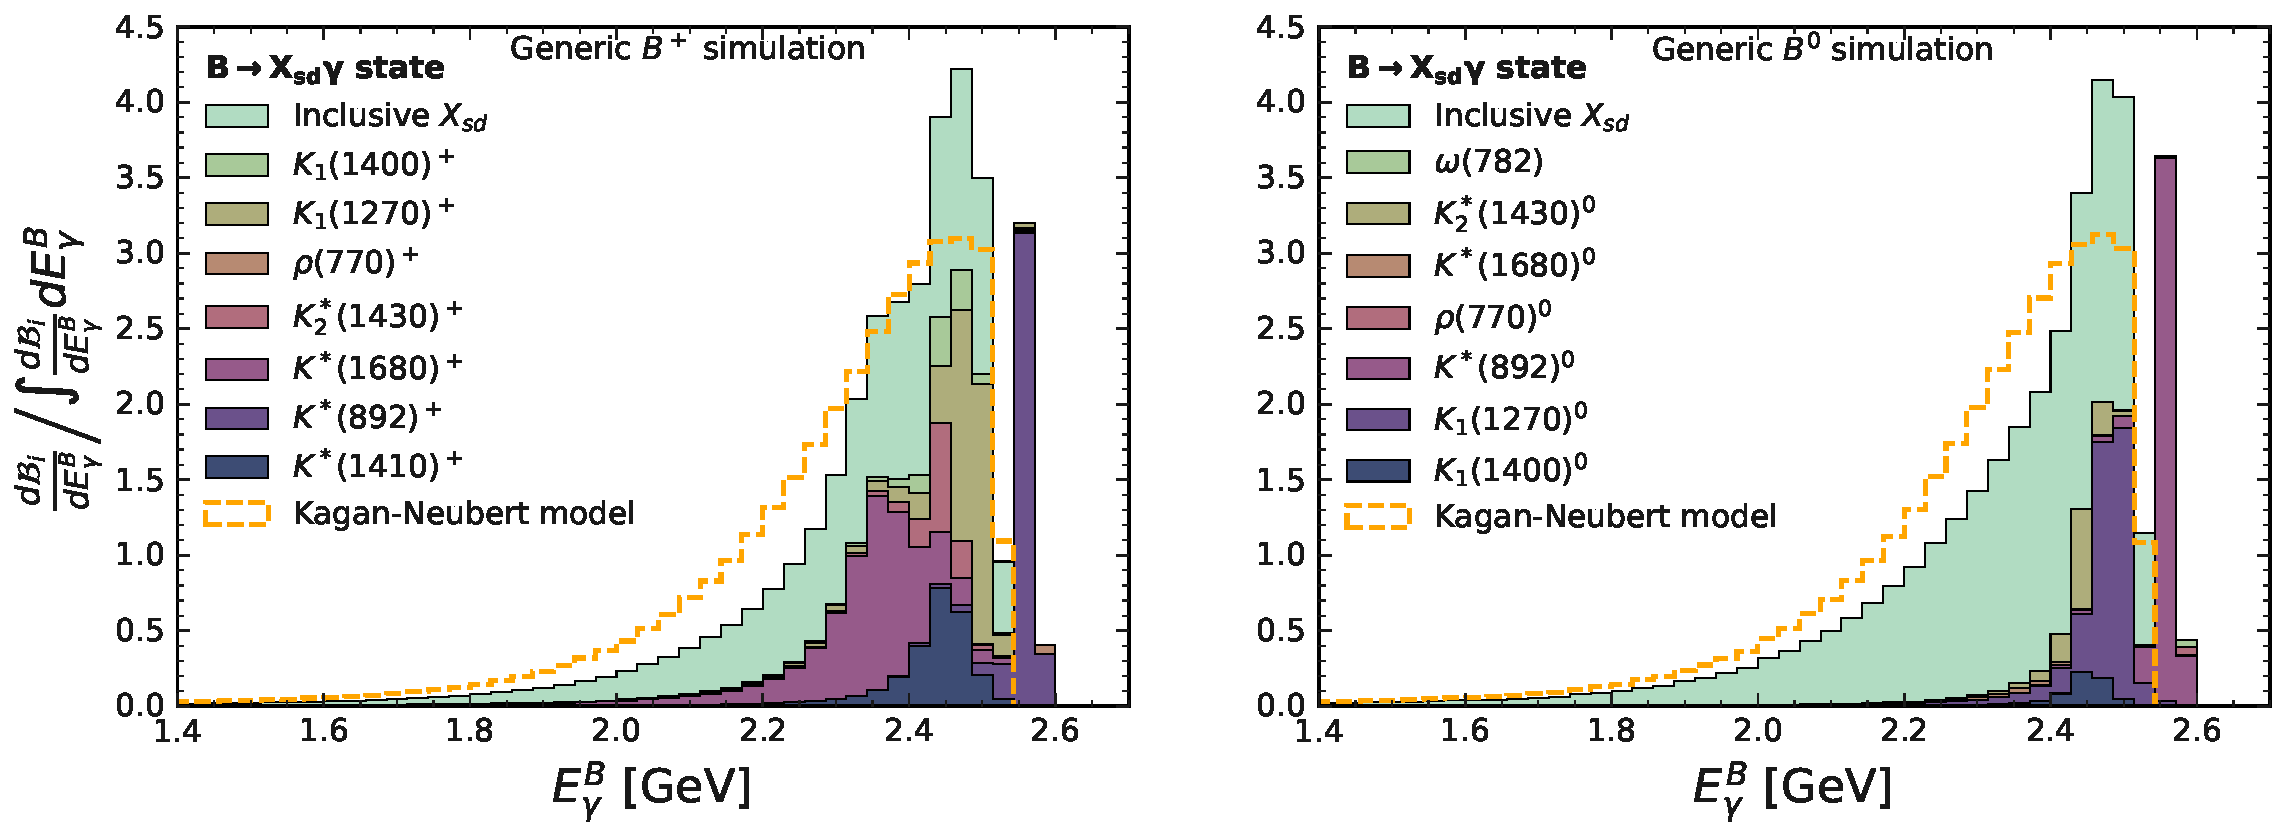
\includegraphics[width=1\textwidth]{figures/data_samples/generic_Xs_simulation.pdf}
    }
    }
    \subcaptionbox{\label{fig:generic_Xsz_model}}{
    \clipbox*{{0.5\width} {0\height} {1\width} {1\height}}{%
    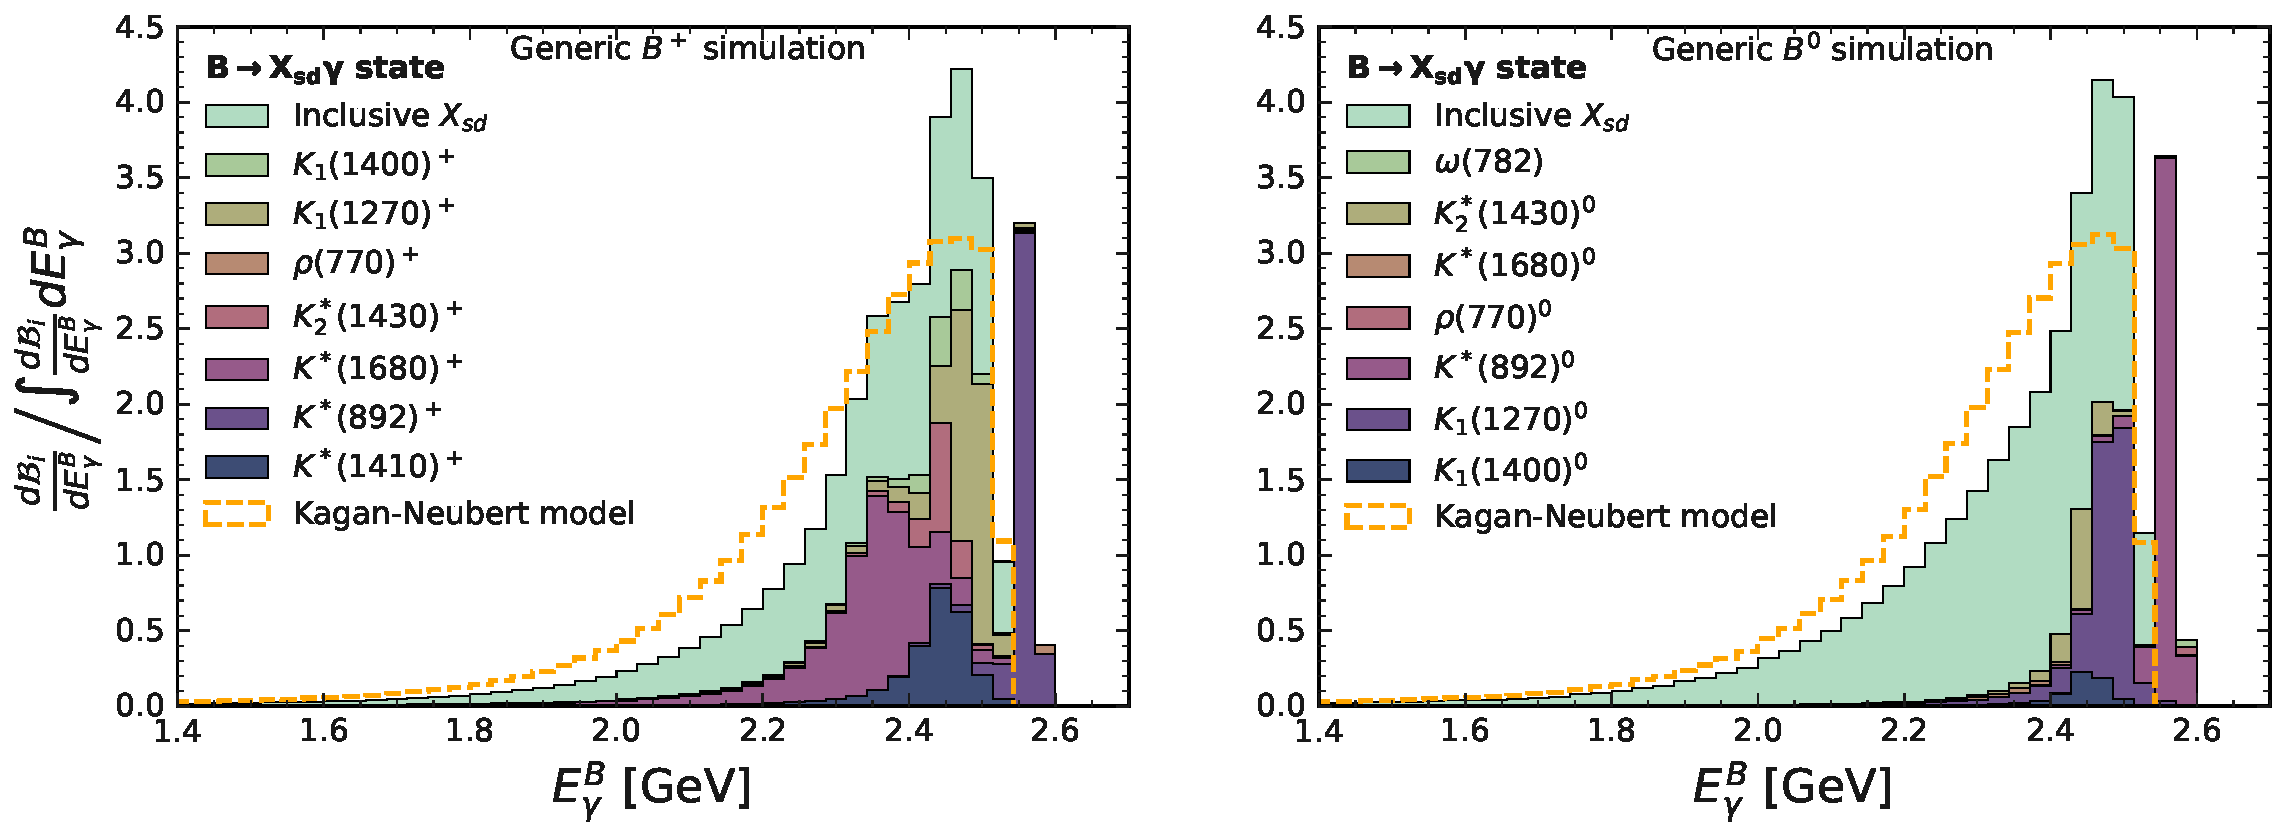
\includegraphics[width=1\textwidth]{figures/data_samples/generic_Xs_simulation.pdf}
    }
    }
    \caption{\label{fig:generic_Xs_model} The model for \BtoXsgamma used in the Belle II official generic-\Bp (\Cref{fig:generic_Xsp_model}) and generic-\Bz (\Cref{fig:generic_Xsz_model}) \MC.
    Althought only several resonances are included, one can see that their individual structure is smoothed out.
    Unknown/unmeasured resonances as well as non-resonant decays are modelled with the inclusive Kagan-Neubert model, but the model is globally scaled down to account for the phase-space covered by the exclusive decays.
    The branching fractions used here are taken from \Cref{tab:btosgamma_bfs} or upper-limits from Refs.\cite{Workman:2022ynf,Amhis:2022mac}.
    The dashed line shows the Kagan Neubert Model.
    The figures are produced using 500 000 event data sets for each mode produced by \texttt{EvtGen} equivalently to Belle II simulation.
    }    
\end{figure}

To ensure that the tail-region is described correctly, while the resonant part is accounted for, a \textit{hybrid model} approach was prepared for this analysis.
It is implemented in a modified approach proposed by Ref.\cite{Ramirez:1989yk}, where it was used for $\B\to X_u\ell\nu$.
The \BtoXsgamma photon-energy spectrum is subdivided in multiple intervals, referred to as \textit{hybrid bins}.
The scaling, called \textit{hybrid weight}, instead of being global, is then calculated for each hybrid bin, such that:
\begin{equation}\label{eq:hybrid_model_definition}
    H_i = I_i\times h_i + \Sigma R_i,
\end{equation}
where $h_i$ is a hybrid weight for hybrid bin $i$; 
$I_i$ is the inclusive model prediction for the given hybrid bin; 
$\Sigma R_i$ is the prediction of all resonances in the hybrid bin;
$H_i$ is the hybrid model prediction in the hybrid bin.

As mentioned before, for the $I_i$ part, Kagan-Neubert model is used (\Cref{sec:btosgamma_spectrum_theory}).
In order to use more up-to-date parameters of the spectrum, the spectrum is reweighted to be compatible with parameters from \Cref{eq:simba_result}.
In the kinetic scheme, compatible with \texttt{EvtGen} implementation of the Kagan-Neubert model, this amounts to:
\begin{equation}\label{eq:simba_result_kinetic}
    m_b^{kin} =4.624~\gevcc \pm 0.045;  \quad \lambda^{\mathrm{kin}}_1 = -0.35\pm0.08,~\gev^2/c^4.
\end{equation}
Taking into account the correlation of these parameters from the determination as described in Ref.\cite{Bernlochner:2020jlt}, 4 additional up and down variations in the eigen directions are generated, which is used as the inclusive model uncertainty in this analysis.
The reweighted inclusive model is shown in \Cref{fig:inclusive_reweighted}.
\begin{figure}[htbp!]
    \centering
    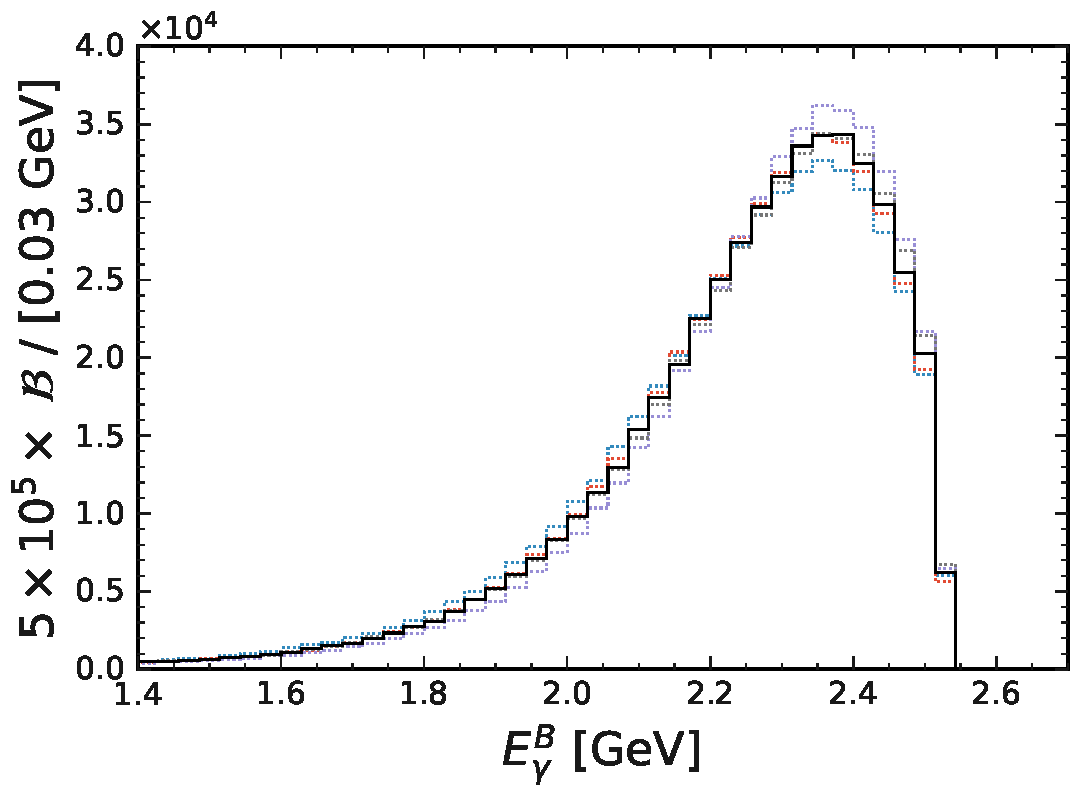
\includegraphics[width=0.45\textwidth]{figures/data_samples/xs_model_inclusive.pdf}
    \caption{\label{fig:inclusive_reweighted}The inclusive $X_s$ model based on \Cref{eq:simba_result_kinetic}.
    The dashed lines show 4 up and down $m_b$ and $\lambda_1$ variations based on their correlated uncertainties.
    The maximum deviations (envelope) is taken as a model uncertainty.}
\end{figure}

For the $R_i$ part, it was decided to include only the $B\rightarrow\Kstar(892)\gamma$ resonance.
The main reason to exclude other resonances is the fact that most are not known precisely, which would lead to a larger modelling uncertainty.
Furthermore, the expected statistical precision (see discussion in \Cref{sec:binning}) is not high enough be sensitive to fine detail in the spectrum.

The set of hybrid bins was selected as displayed in \Cref{fig:hybrid_bins_and_model}.
An underflow and overflow bin is selected at $1.6$ and $2.3~\gev$, respectively.
The overflow bin is chosen to include the majority extent of the $\B\to\Kstar(892)\gamma$ resonance.
The finer 0.1~\gev-wide bins in between contain small amounts of $\B\to\Kstar(892)\gamma$ events.
In each \EB bin, an appropriate hybrid weighth is calculated, such that the sum of the reweighted inclusive model (\Cref{fig:inclusive_reweighted}) and $\B\to\Kstar(892)\gamma$ contribution matches the partial branching fraction within that \EB bin, based on \Cref{eq:hybrid_model_definition}.
This captures the desired description of the low-\EB region with the inclusive model, and a \Kstar(892) resonance-dominated behaviour at high-\EB.

\begin{figure}[htbp!]
    \subcaptionbox{\label{fig:hybrid_binned_model}}{%
        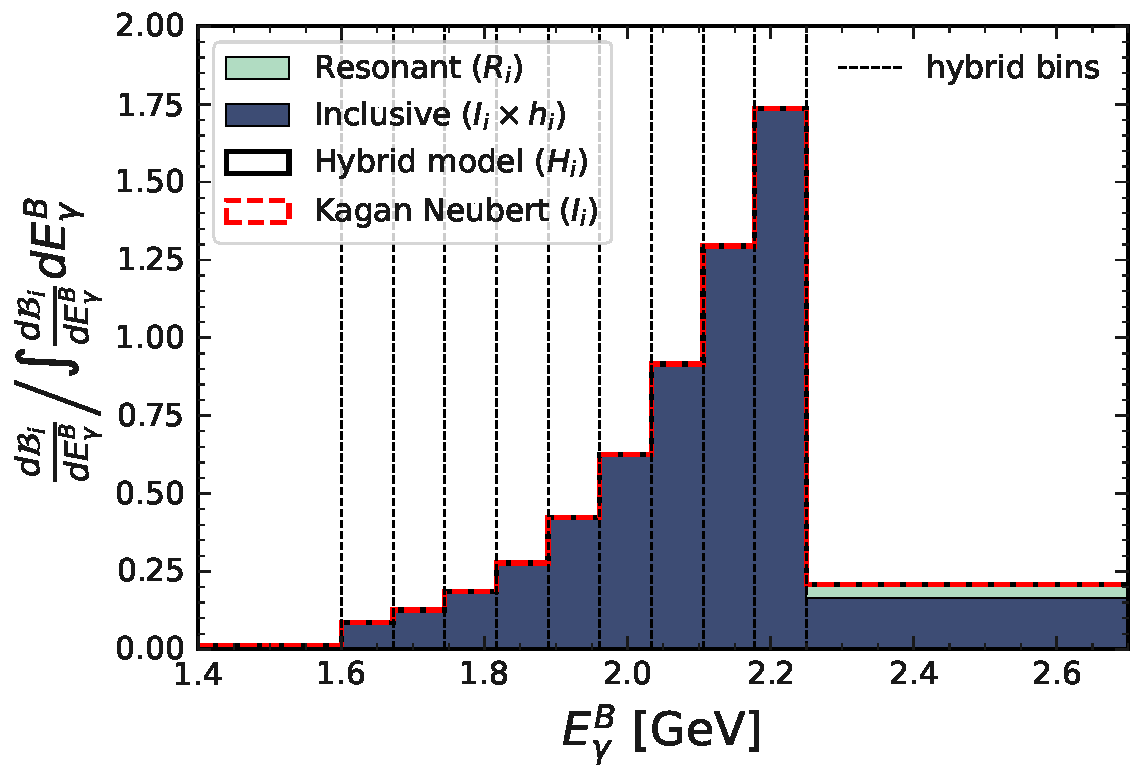
\includegraphics[width=0.45\textwidth]{figures/data_samples/normalised_signal_model_hybrid_binning.pdf}
    }
    \subcaptionbox{\label{fig:hybrid_binned_analysis_model}}{%
        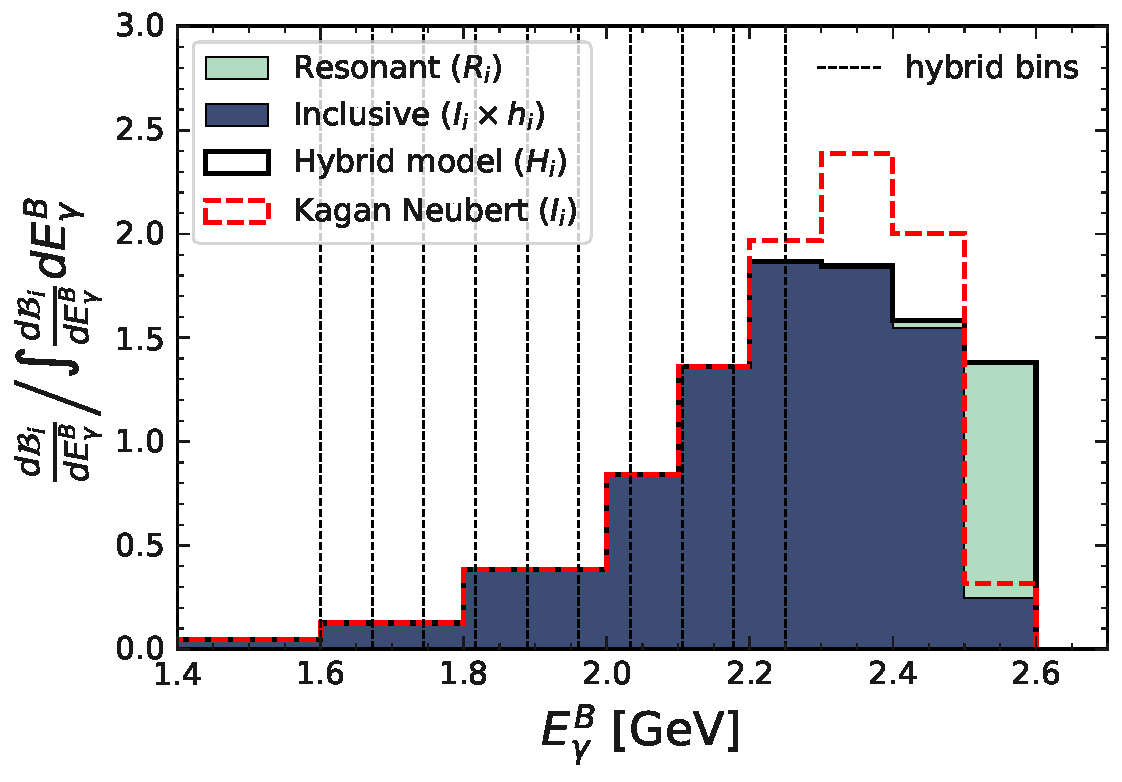
\includegraphics[width=0.45\textwidth]{figures/data_samples/normalised_signal_model.pdf}
        }
    \caption{\label{fig:hybrid_bins_and_model} Hybrid model construted for this analysis 
    shown in two different binnings.
    \Cref{fig:hybrid_binned_model} shows it for a binning that matches the hybrid-binning; 
    and \Cref{fig:hybrid_binned_analysis_model} shows it for a binning that will 
    be chosen in this analysis (see \Cref{sec:binning} and \Cref{tab:expected_events}).
    In both cases, the spectra are normalised such that the total area under them is 1.
    It is clear, that the hybrid model describes the tail adequatly, 
    while also taking into account the resonant contributions (compare with \Cref{fig:generic_Xs_model}).
    The different components corresponding to \Cref{eq:hybrid_model_definition} are labelled appropriately.
    }
\end{figure}

The hybrid bins need not match the binning used in the analysis or plotting.
As seen in \Cref{fig:hybrid_binned_analysis_model}, the hybrid model can be used for different binnings which do not coincide with the hybrid bins.
In the figure, the model is shown in the binning that will later be used for the analysis, after optimising based on expected signal and background contributions.

The uncertainty of the hybrid model is evaluated taking into account:
\begin{itemize}
    \item Branching fraction uncertainty of the $\B\to\Kstar(892)\gamma$, $\sigma_{\mathrm{res}}$;
    \item Branching fraction uncertainty of the inclusive \BtoXsgamma decay, $\sigma_{\mathrm{incl}}$;
    \item Inclusive model parameter variations, as shown in \Cref{fig:inclusive_reweighted}, $\sigma_{\mathrm{var}}$.
\end{itemize}
These components are evaluated based on the values discussed in this Section and given \Cref{tab:btosgamma_bfs}.
They are visually shown for a selected \BtoXsgamma photon-energy spectrum binning in \Cref{fig:hybrid_uncertainty}.
The uncertainty is dominated by \BtoXsgamma model variation uncertainties, except in the interval where $\B\ra\Kstar(892)\gamma$ dominates, where its branching fraction uncertainty is dominant.
The uncertainty related to the \BtoXsgamma inclusive branching fraction model is much smaller than the other two.
\begin{figure}[htbp!]
    \centering
    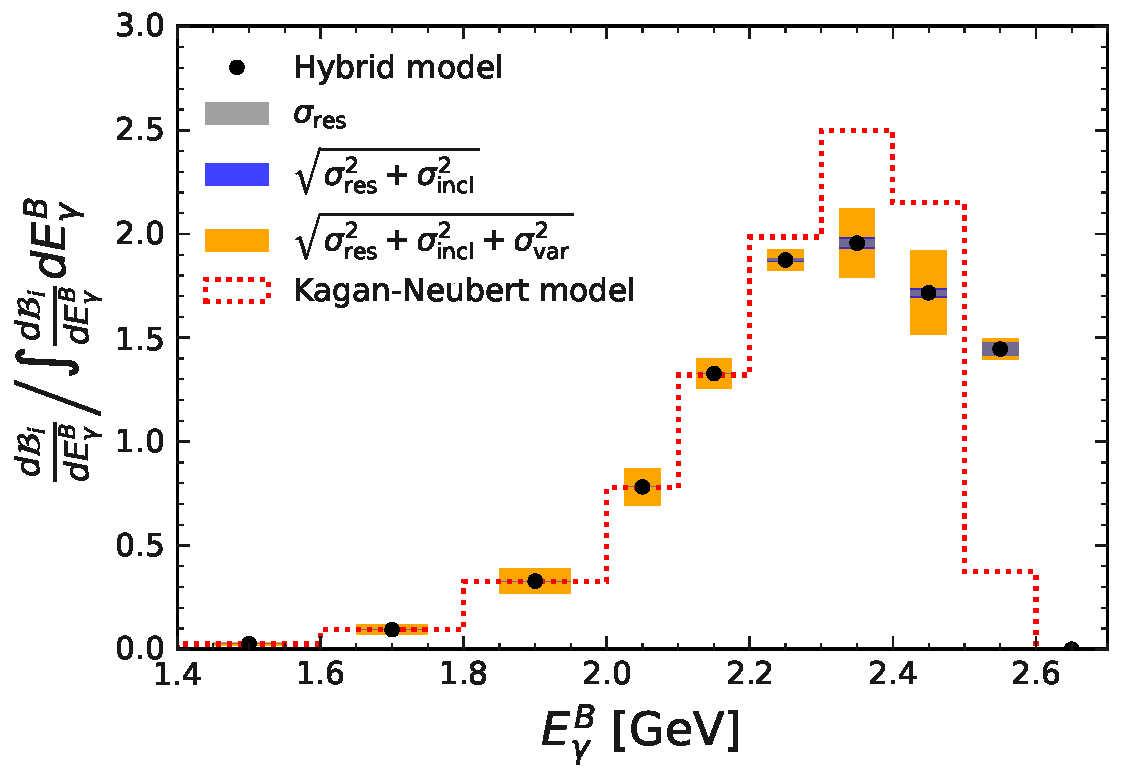
\includegraphics[width=0.45\textwidth]{figures/data_samples/hybrid_model_uncertainties.pdf}
    \caption{\label{fig:hybrid_uncertainty}The inclusive $X_s$ model based on \Cref{eq:simba_result_kinetic},
    with uncertainties from the resonant, inclusive branching fractions and the inclusive model parameters overlaid.
    The definitions of uncertainties are given in the text.
    For comparison, the Kagan-Neubert model with the same parameters is also shown.
    }
\end{figure}


